\section{Language Evaluation Criteria}
In this section the different criteria proposed in \cite{sebesta1.3} are presented. These criteria are used to facilitate the design of \lang{}.
The three main aspects of a language, according to \cite{sebesta1.3}, are \textit{Readability, Writability and Reliability}. These have a list of criteria which is applicable to the main aspects:
\begin{figure}[H]
    \centering
    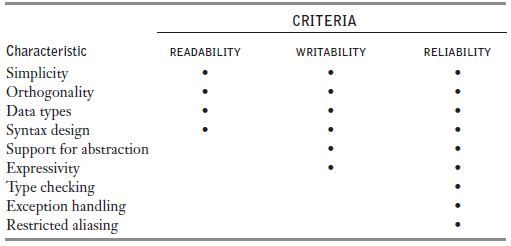
\includegraphics[scale=1]{resources/Images/criteria.PNG}
    \caption{Table from \cite{sebesta1.3} with the different criteria, and how they affect aspects of the language.}\label{fig:Criteria}
\end{figure}
The following sections briefly summarise the aspects covered by the above-mentioned criteria.
\newpage
\subsection{Readability}
An important aspect of a beginner-friendly programming language is that it has to be easily readable. When considering the readability, the problem-domain also has to be drawn in, as a language could be readable when used for writing games, which is the main domain of the language, but difficult to read when used for writing something not in the domain of the language.
\subsubsection{Simplicity}
The simplicity of a language has to take into account 3 important aspects:
\begin{itemize}
    \item \textbf{Language constructs}:\\
     A language with a large amount of constructs can be hard to remember, and in reality, a lot of programmers might learn a subset of the total amount of features of a language, instead of learning the language as a whole.
    \item \textbf{Feature multiplicity}:\\
     Having multiple ways to accomplish the same thing can be confusing and hard to read, especially for beginners. The fact that something can be done in many different ways is bad for the readability, because it might not be what this particular programmer expects to see when he reads a program.
    \item \textbf{Operator overloading}:\\
    One operator symbol meaning multiple things can lead to bad readability. The meaning of operators are typically clear and easy to understand, but if an operator is suddenly overloaded to do something else based on the context, it can become harder to read.
\end{itemize}
\subsubsection{Orthogonality}
Orthogonality means that the ways in which the primitive constructs of the language can be combined together, is relatively small, and the combinations that do exist, are meaningful. This is important when programming, because if the orthogonality is too low, the usage of the different combinations will not make sense to the programmer. This is because too many exceptions in how the programming language works, confuses the programmer, thus making it nonsensical. 
\subsubsection{Syntax Design}
Regarding the design of the syntax of a language, one should take two important aspects into account:
\begin{itemize}
    \item \textbf{Reserved words}:\\
    These constitute words such as:
    \begin{itemize}
        \item \textit{while}
        \item \textit{if}
        \item \textit{for}
    \end{itemize}
    If the reserved word used to do control structures such as these are not named in a meaningful way, the reader may find it difficult to understand the semantics of a piece of code.
    \item \textbf{Form and meaning}:\\
    This sub-criterium refers to the idea that the behavior of the statements should somehow be self-explanatory to aid readability. 
\end{itemize}
\subsubsection{Data Types}
There should be sufficient data types to support most common tasks in programming, as this makes it easier and faster to program, since the programmers do not have to define new types themselves.
\subsection{Writability}
The second important aspect for a beginner friendly language is that it should be easy to write. This does not necessarily mean that it has to be simple or written with few words, but more so that it has to be easy to understand how to write code. This is achieved by fulfilling a number of criteria, listed in the next couple of sections.
\subsubsection{Simplicity and orthogonality}
When beginners begin to learn how to use and write programs in a new language, they will not know all of the different constructs available in the language. This can lead to programs that perform poorly or programs that are simply wrong. This is because the beginners will use the constructs they know, or can intuitively understand, and not the more advanced or unknown ones.
\subsubsection{Support for Abstraction}
It is important in any programming language that there is proper support for abstraction. Otherwise programs in the language are complicated to read. The creation of new programs will take longer, and the maintainability of the programs would become more difficult and error prone. A beginner is not going to be too concerned with maintainability, but the concept of abstraction over certain parts of a program via the use of, among others, methods/subroutines data structures, is a very concept of programming languages in general that a beginner needs to get used to. A language with good support for abstraction will also feel more natural to write in. 
\subsubsection{Expressivity}
This criteria simply refers to the fact that the language should have convenient ways of expressing complex computations.
\subsection{Reliability}
Reliability is about whether or not a program performs how it should under all kinds of conditions. The following sections presents the main aspects that contribute to making a language reliable.
\subsubsection{Type Checking}
A language designed for beginners should have static type checking as opposed to dynamic type checking. Such a language should be designed to guide and help beginners, and having dynamic type checking leaves a lot of type casting errors to be found by the programmer while executing the program. These errors can be particularly hard to debug in advance. 
\subsubsection{Exception Handling}
Exception handling is about the language's ability to catch errors thrown during execution. In a beginner language, this feature is not the most important feature, but it is still needed, because it is in general impossible to avoid situations where errors are thrown. Especially when dealing with I/O features typical of gaming.
\subsubsection{Aliasing}
Aliasing refers to the fact that two or more names can be used to access the same memory cell. This is not recommended for a beginner language because it leads to confusion about what names refer to what. 
\subsubsection{Readability and Writability}
The reliability of a language is greatly influenced by the two other aspects: readability and writability. A language that is very readable and easily writable has a much better chance of having a user producing programs that run correctly and efficiently. This is assuming that the language itself is not written inefficiently.
\subsection{Cost}
There is a fourth aspect which is about the cost of writing in the language in terms of development time and general resource usage. The cost in terms of time is not important to someone just beginning to learn a language, but there is a couple of other aspects worth considering when considering cost of using a beginners language.
\subsubsection{Training programmers}
This criteria concerns whether or not the language is good at teaching beginners the constructs of programming languages. A language that has a low cost in terms of training programmers has intuitive and simple constructs that help the beginner to understand the purpose of said constructs.
\subsubsection{Compiler efficiency}
Compiler efficiency concerns how fast the compiler compiles a source program and how optimized the translation into the target language is.

%or not the compiler is efficient and/or fast to use. A compiler that is hard to use will hurt the cost of the language, as the user will have to spend more time learning how to compile with it.

\subsubsection{Program Execution}
Program execution concerns the execution speed of the program. A beginner friendly language, for making games, is not going to be overly concerned with the execution speed, but it should still not have any noticeable slowdowns. A beginner friendly programming language should, however, be able to run fluent graphics without the user having any knowledge of the technical aspects of graphics.
\newpage

\section{Language Evaluation of \lang{}}
This chapter rates the above-mentioned criteria after how important they are for \lang{}, and motivates the reason for such ratings. The ratings are shown in a priority table presented in the following table:

\begin{table}[H]
\centering


\begin{tabular}{|l|c|c|c|c|}
\hline
\rowcolor[HTML]{EFEFEF} 
                        & Very important & Important  & Less important & Unimportant \\ \hline
\rowcolor[HTML]{34CDF9} 
Simplicity              & \textbf{X}     &            &                &             \\ \hline
\rowcolor[HTML]{BBDAFF} 
Orthogonality           &                &            & \textbf{X}     &             \\ \hline
\rowcolor[HTML]{34CDF9} 
Data types              &                & \textbf{X} &                &             \\ \hline
\rowcolor[HTML]{BBDAFF} 
Syntax design           & \textbf{X}     &            &                &             \\ \hline
\rowcolor[HTML]{34CDF9} 
Support for abstraction & \textbf{X}     &            &                &             \\ \hline
\rowcolor[HTML]{BBDAFF} 
Expressivity            &                & \textbf{X} &                &             \\ \hline
\rowcolor[HTML]{34CDF9} 
Type checking           &                & \textbf{X} &                &             \\ \hline
\rowcolor[HTML]{BBDAFF} 
Exception handling      &                &            & \textbf{X}     &             \\ \hline
\rowcolor[HTML]{34CDF9} 
Restricted aliasing     &                &            &                & \textbf{X}  \\ \hline
\rowcolor[HTML]{BBDAFF} 
Teaching programmers    & \textbf{X}     &            &                &             \\ \hline
\rowcolor[HTML]{34CDF9} 
Writing programs        &                &            & \textbf{X}     &             \\ \hline
\rowcolor[HTML]{BBDAFF} 
Compiler efficiency     &                &            & \textbf{X}     &             \\ \hline
\rowcolor[HTML]{34CDF9} 
Program execution       &                & \textbf{X} &                &             \\ \hline
\end{tabular}
\label{tab:criteria}
\caption{Criteria prioritizing table.}
\end{table}

The reasons for the different prioritisations in the table is described in the following sections. 

\subsection*{Simplicity}
As \lang{} is meant to be a beginner friendly language rather than a professional language, the simplicity is very important. The simplicity is held high by reducing the amount of constructs to as few as possible. For example, all number types are merged into one type called \textit{num}. Furthermore, \textit{char} and \textit{string} are merged into \textit{text}. \\
Apart from having fewer language constructs, there are little to no feature multiplicity. For example, \lang{} does not allow the user to use expressions such as \textit{x++} in place of \textit{x = x+1} like a number of other programming languages.
The last thing done to keep the simplicity up is making operators and reserved words only mean one thing. For example, '=' is only used as a boolean equals, whereas in other languages '=' has been used to assign a variable to a value, and '=='s are used as a boolean equals.

\subsection*{Orthogonality}
Orthogonality is less important for this project, as it is relatively low in \lang{}. Even though it is possible to create custom datatypes, they can only be combined in logical ways, such as inheritance and composition. 

\subsection*{Data types}
Data types are important for \lang{} as readability has a high priority. This is seen in for example "bool" and "text", where they both will have more intuitive names rather than just "bool" being either 1 or 0, and "text" being "string". 

\subsection*{Syntax design}
Syntax design is very important. To keep up the readability, english words have been preferred over symbols for many reserved words. For example, declaration looks like this in C\# and Java: \texttt{\textcolor{red}{int} x = 1} but like this in \lang{}: \texttt{\textcolor{blue}{dcl} \textcolor{pink}{num} x \textcolor{blue}{to} 1}. The purpose of this is to make it easier for new programmers to read the code, as it is written more like how it is said.

\subsection*{Support for abstraction}
Support for abstraction is one of the essential parts of \lang{}. This is seen in, among others, our primitive constructs. The user does not have to know whether a number is an int32 or int64. It does not even have to know whether it is an int or a float. Same goes with chars and string, which both goes under the same construct called text.

\subsection*{Expressivity}
Expressivity is important for \lang{}. It is important that the programmer is able to make complex code easily. For example, it is possible to do graphics with just a few lines of code.

\subsection*{Type checking}
Type checking in \lang{} is important because it is important for making languages reliable. \lang{} implements static type checking, so that the user will be warned about type errors at compile time.

\subsection*{Exception handling}
\lang{} Does not support constructs for handling or throwing exceptions. However, exceptions may be thrown, when running the code. In this case, the user is notified about the reason why the exception has occurred. Exception handling is therefore less important. 

\subsection*{Restricted aliasing}
Aliasing may be confusing to beginners. For this reason, aliasing is restricted to object references, and can be made only through reference variables. Pointers are not allowed. Therefore, Restricted aliasing is unimportant for \lang{}. 

\subsection*{Training new programmers} 
As previously stated, \lang{} is a language specifically made to teach people, who are new to textual programming, to program this way. Therefore, is this part very important. %To this end, the language will be supported with tutorials. Wat?

\subsection*{Writing programs}
Also as previously stated, \lang{} is not meant to be used to make programs in an effective manner, but rather creating small programs to get the hang of textual programming. 

\subsection*{Compiler efficiency}
It does not really matter how efficient the compiler is for \lang{}, as there will only be written small programs in it, which a very good compiler efficiency only would affect by a very small margin. Therefore, compiler efficiency is less important.

\subsection*{Program execution}
Program execution is important because the programmer should not experience lag or waiting time while executing a compiled game. The compiled game should run smoothly, and the compiling process should not be too lengthy. The last point is remedied by the fact that games in \lang{} should be written in relatively few lines of code, and as such will not take a long time to compile, even with a relatively inefficient compiler. 

To further analyze which of the above points are essential, it was choosen to perform a MosCoW analysis. This analysis is described in the next chapter. 